% !TeX program = pdflatex
% Standalone source: arxiv_en.tex. Figure and bibliography are embedded.
\documentclass[11pt,a4paper]{article}
\usepackage[T1]{fontenc}
\usepackage[utf8]{inputenc}
\usepackage[english]{babel}
\usepackage{lmodern}
\usepackage[margin=1in]{geometry}
\usepackage[numbers,sort&compress]{natbib}
\usepackage{amsmath,amssymb,amsthm}
\usepackage{tikz}
\usepackage{microtype}
\usepackage{xurl}
\usepackage[hidelinks]{hyperref}
\newtheorem{theorem}{Theorem}[section]
\newtheorem{lemma}[theorem]{Lemma}
\newtheorem{corollary}[theorem]{Corollary}
\theoremstyle{remark}
\newtheorem{example}[theorem]{Example}
\numberwithin{equation}{section}
\hypersetup{
  pdftitle={Trees with perfect matchings that disprove a conjecture of Ramos and Sun},
  pdfauthor={Heshun Fan},
  pdfkeywords={Independence polynomial, tree, log-concavity, perfect matching},
  pdfdisplaydoctitle=true
}

\title{Trees with perfect matchings that disprove a conjecture of Ramos and Sun}
\author{Heshun Fan\\
{\small School of Mathematics and Statistics}\\
{\small Huazhong University of Science and Technology}\\
{\small Wuhan 430074, China}\\
{\small \href{mailto:U202410055@hust.edu.cn}{U202410055@hust.edu.cn}}}
\date{}

\begin{document}
\maketitle

\begin{abstract}
We construct an explicit family of trees with perfect matchings whose
independence sequences fail log-concavity one position below the
independence number. For every integer $p\geq6$, the tree has $14p+6$
vertices and independence number $m=7p+3$, while its independent-set
counts satisfy $a_{m-1}^2<a_{m-2}a_m$. This disproves Conjecture~4.2
of Ramos and Sun, which predicts a lower bound on the independence
number from the position of a failure of log-concavity. The proof
encodes independent sets by endpoint choices on matching pairs and
compares counts obtained by deleting pair labels. It also gives
$a_{m-1}^2/(a_{m-2}a_m)<49\cdot2^{-p}$. We give exact coefficients
for the 90-vertex instance and describe its Lean formalization.
\end{abstract}

\begingroup\small
\noindent\textbf{Keywords:} Independence polynomial; tree; log-concavity; perfect matching.\par
\noindent\textbf{2020 Mathematics Subject Classification:} 05C31, 05C05, 05C69, 03B35.\par
\endgroup

\section{Introduction}\label{sec:introduction}

For a finite graph $G$, let $a_k(G)$ denote the number of independent
vertex sets of cardinality $k$, and let $\alpha(G)$ denote its
independence number. The independence polynomial is
\[
 I_G(x)=\sum_{k=0}^{\alpha(G)}a_k(G)x^k.
\]
The sequence is log-concave at an interior index
$1\leq j<\alpha(G)$ if
$a_j(G)^2\geq a_{j-1}(G)a_{j+1}(G)$.
All coefficients from $a_0(G)$ to $a_{\alpha(G)}(G)$ are positive,
since subsets of a maximum independent set realize every such size.
Consequently, log-concavity implies unimodality. These two shape
properties have motivated the study of independence polynomials of
trees; see the background in Ramos and Sun~\cite[Section~2.1]{RamosSun2025}.
Trees with non-log-concave independence sequences are already known
\cite{KadrawiLevit2023}. A more specific question asks how the position
of a failure constrains the independence number.

Put $h=\lfloor N/2\rfloor$ for a tree $T$ of order $N$.
Motivated by their computational searches, Ramos and Sun proposed
the following implication in Conjecture~4.2 of~\cite{RamosSun2025}:
\begin{equation}
 a_{h-\beta}(T)^2<a_{h-\beta-1}(T)a_{h-\beta+1}(T)
 \quad\Longrightarrow\quad
 \alpha(T)\geq h+\beta+1.
 \label{eq:conjecture}
\end{equation}
Their convention in Section~1.2 replaces $N/2$ by its floor when
$N$ is odd. The conjecture does not separately specify a range for
$\beta$. We disprove the even-order case with $\beta=1$ and with
all three coefficient indices in the positive support.
In this case, failure at $N/2-1$ would require
$\alpha(T)\geq N/2+2$.

Every tree of order $N$ has independence number at least
$\lceil N/2\rceil$, by its bipartition. For a tree of order $2m$
with a perfect matching, each independent set uses at most one
endpoint of each matching edge, while each bipartition class has
size $m$. Such a tree therefore has independence number exactly $m$.
Our construction attains this value and fails log-concavity at $m-1$.
Write $\nu(G)$ for the maximum size of a matching in $G$.

\begin{theorem}\label{thm:main}
For each integer $p\geq6$, construct $T_p$ from six distinct vertices
$a,b,c,d,e,f$ with edges
\[
 ab,\quad cd,\quad ef,\quad af,\quad cf
\]
by attaching $p$ pendant paths of length two at each of $a,c,e$, and
$2p$ such paths at each of $b,d$. Each attached path has two new
vertices, distinct from those of every other attached path.
Then $T_p$ is a tree with
\[
 |V(T_p)|=14p+6,\qquad \nu(T_p)=\alpha(T_p)=7p+3.
\]
Writing $m=7p+3$ and $a_k=a_k(T_p)$, we have
\begin{equation}
 a_{m-1}^2<a_{m-2}a_m.
 \label{eq:failure}
\end{equation}
Thus $T_p$ contradicts~\eqref{eq:conjecture} with $\beta=1$.
\end{theorem}

Indeed, the conjecture would require $\alpha(T_p)\geq m+2$,
whereas $\alpha(T_p)=m$. The proof also shows that
$a_{m-1}^2/(a_{m-2}a_m)<49\cdot2^{-p}$, so this ratio tends to zero
along the family; see Corollary~\ref{cor:ratio}.
For $p=6$, we obtain a 90-vertex counterexample with independence
number $45$ and failure at index $44$.

The matching has a second role beyond fixing the independence number.
An independent set leaves some matching pairs empty and selects one
endpoint of each remaining pair. Thus the three highest-degree
coefficients count configurations with zero, one, and two empty pairs.
Attaching paths of length two preserves the matching, and the unequal
numbers $p$ and $2p$ of attached paths give different weights to the
two endpoint choices in a core pair. Leaving two specified core pairs
empty removes the restrictions on many pendant pairs at once.
This gives a lower bound for $a_{m-2}$ that, when multiplied by $a_m$,
exceeds the square of the sum of all one-empty-pair contributions. Only a few
exact counts are needed; the remaining contributions admit a common
bound.

\subsection{Relation to earlier constructions}\label{sec:related}

To compare an established failure at index $j$ with the proposed
bound~\eqref{eq:conjecture}, set $\beta=h-j$. The proposed conclusion
then reads
\begin{equation}\label{eq:comparison-test}
 \alpha+j\geq2\lfloor N/2\rfloor+1.
\end{equation}
The comparisons below concern the specific failure indices established
in the cited works. When $j>h$, this substitution gives a negative
$\beta$ rather than an instance with nonnegative $\beta$.

Kadrawi and Levit~\cite[Sections~3--4]{KadrawiLevit2023} give two
types of infinite families extending their 26-vertex examples.
The stated failures have $\alpha=N/2+1$ and $j=N/2$, so
\eqref{eq:comparison-test} holds with equality.
Galvin~\cite[Theorem~2.1]{Galvin2026} constructs trees $T_{q,t,1}$ with
\[
 N=1+q+2qt,\qquad \alpha=q(t+1),\qquad j=qt+2
\]
for integers $t\leq q\leq2^{t/16}$ and sufficiently large $t$.
Here $\alpha+j=N+1$, which implies~\eqref{eq:comparison-test}.
Both types of Kadrawi--Levit trees and Galvin's trees have
$\alpha>N/2$, in contrast to Theorem~\ref{thm:main}.

Bautista-Ramos~\cite[Definition~1 and Theorem~1]{BautistaRamos2025}
constructs trees with arbitrarily many failures. Denoting the number
of branches by $q$, the parameters are
\[
 N=2+q(4+6t),\qquad \alpha=1+3q(t+1),\qquad
 j=\alpha-(2r+1),
\]
where $q\geq1$ is a fixed integer, $t$ is a sufficiently large
integer, and $r\in\{0,\ldots,q-1\}$. In this case,
$\alpha+j-N-1=2(q-r-1)\geq0$, and
$\beta=1-q+2r$ is nonnegative precisely when $2r\geq q-1$.
Bautista-Ramos, Guill\'en-Galv\'an, and G\'omez-Salgado~\cite{BGG2026}
develop rooted constructions and linear recurrences with consecutive
failures. Their Corollary~4 gives
$(N,\alpha,j)=(19q+6,10q+3,10q+2)$ for integers $q\geq9$.
These parameters satisfy~\eqref{eq:comparison-test}, since
$\alpha+j-N-1=q-2>0$, but give
$\beta=1-\lceil q/2\rceil<0$.
Galvin~\cite[Section~3]{Galvin2026} also reports examples computed by
Bencs with several failures, without specifying their indices;
those data do not determine the comparison in~\eqref{eq:comparison-test}.

In a September 2026 preprint, Fang, Lu, Nevo, Yao, and
Zheng~\cite[Theorems~1.1--1.2]{Fang2026} announce unimodality for
sufficiently large forests and strict log-concavity in the range
$N/5\leq j\leq17\alpha/25$.
Our index $j=\alpha-1$, with $\alpha\geq45$, lies beyond that range.
The local failure in Theorem~\ref{thm:main} does not imply a failure
of unimodality.

The representation of a tree by matching pairs and oriented edges
also occurs in the public implementation~\cite{MatchingLift}.
Public Lean source~\cite{LeanWitnesses} contains a correctness theorem
linking rooted-tree polynomial calculations to independent-set
counts, together with non-log-concave witnesses of orders $26$, $28$,
and $29$. The two even-order witnesses have
$(N,\alpha,j)=(26,14,13)$ and $(28,15,14)$, and hence satisfy
\eqref{eq:comparison-test}; the odd-order witness has
$j=15>\lfloor29/2\rfloor$.
The formalization described here concerns the 90-vertex instance of
Theorem~\ref{thm:main}.

\noindent\textbf{Organization.}
Section~\ref{sec:proofs} proves Theorem~\ref{thm:main} by counting
assignments on matching pairs and derives the bound on the coefficient
ratio. Section~\ref{sec:formalization} gives the exact 90-vertex
instance and the scope of its formal verification.
Section~\ref{sec:discussion} discusses the parameter threshold and
further coefficient estimates. Appendix~\ref{app:verification}
records an independent polynomial recurrence and the formal source
identifiers.

\noindent\textbf{Conventions and notation.}
All graphs are finite and simple. The length of a path is its number
of edges. Vertex deletion is induced deletion, and $N_G[v]$ denotes
the closed neighborhood of $v$. We set $a_k(G)=0$ for
$k>\alpha(G)$ and $I_{\varnothing}(x)=1$.

\section{Counting independent sets through a perfect matching}\label{sec:proofs}

We prove Theorem~\ref{thm:main} by using the perfect matching to count
independent sets. The matching first determines the independence number;
the resulting representation of independent sets then reduces the
coefficient comparison to counts on a directed tree of matching pairs.

\subsection{The tree and its matching pairs}\label{sec:construction}

Fix an integer $p\geq6$, put $m=7p+3$, and abbreviate
$a_k=a_k(T_p)$ for the rest of the proof.
The six-vertex core is connected with five edges, hence is a tree.
Attaching a path with two new vertices preserves connectedness and
acyclicity. There are $7p$ attached paths, so the resulting tree has
$6+14p=2m$ vertices. The three core edges $ab,cd,ef$, together with
the outer edge of every attached path, form a perfect matching of
size $m$; see Figure~\ref{fig:core}. Thus $\nu(T_p)=m$.

\begin{figure}[ht]
\centering
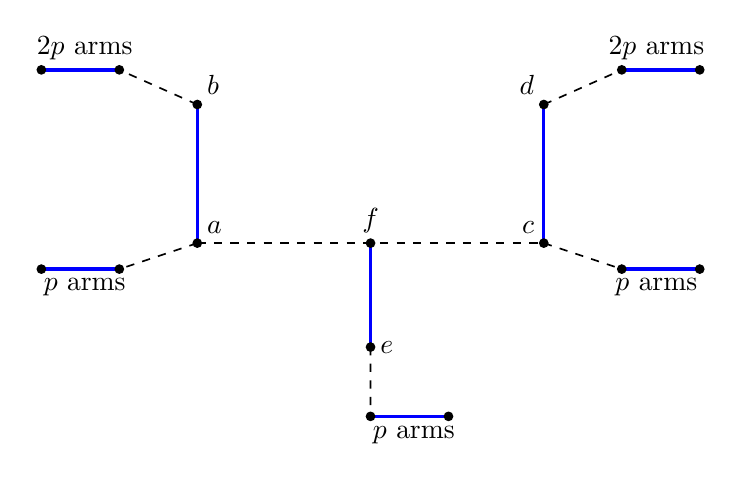
\begin{tikzpicture}[scale=1.1]
\coordinate (a) at (-2,0);
\coordinate (b) at (-2,1.6);
\coordinate (c) at (2,0);
\coordinate (d) at (2,1.6);
\coordinate (e) at (0,-1.2);
\coordinate (f) at (0,0);
\coordinate (a1) at (-2.9,-.3);
\coordinate (a2) at (-3.8,-.3);
\coordinate (b1) at (-2.9,2);
\coordinate (b2) at (-3.8,2);
\coordinate (c1) at (2.9,-.3);
\coordinate (c2) at (3.8,-.3);
\coordinate (d1) at (2.9,2);
\coordinate (d2) at (3.8,2);
\coordinate (e1) at (0,-2);
\coordinate (e2) at (.9,-2);
\draw[black,line width=0.6pt,dashed] (a)--(f)--(c);
\draw[black,line width=0.6pt,dashed] (a)--(a1) (b)--(b1) (c)--(c1) (d)--(d1) (e)--(e1);
\draw[blue,line width=1.2pt] (a)--(b) (c)--(d) (e)--(f);
\draw[blue,line width=1.2pt] (a1)--(a2) (b1)--(b2) (c1)--(c2) (d1)--(d2) (e1)--(e2);
\foreach \v in {a,b,c,d,e,f,a1,a2,b1,b2,c1,c2,d1,d2,e1,e2}
  \fill (\v) circle (1.6pt);
\node[above right] at (a) {$a$};
\node[above right] at (b) {$b$};
\node[above left] at (c) {$c$};
\node[above left] at (d) {$d$};
\node[right] at (e) {$e$};
\node[above] at (f) {$f$};
\node[below] at (-3.3,-.3) {$p$ arms};
\node[above] at (-3.3,2) {$2p$ arms};
\node[below] at (3.3,-.3) {$p$ arms};
\node[above] at (3.3,2) {$2p$ arms};
\node[below] at (.5,-2) {$p$ arms};
\end{tikzpicture}
\caption{The six-vertex core and one representative of each group of
pendant paths. Each displayed arm represents the stated number of
distinct copies. Thick solid blue edges form the perfect matching;
thin dashed black edges are nonmatching. No arm is attached at $f$.}
\label{fig:core}
\end{figure}

Label the endpoints of the core matching edges by
\[
 (a,b)=(U_u,V_u),\quad (c,d)=(U_v,V_v),\quad
 (e,f)=(U_z,V_z).
\]
Extend the bipartition along every attached path, using $U$ and $V$
for its two classes. Each matching pair is then $\{U_i,V_i\}$ for
some label $i$. The $m$ vertices $U_i$ form an independent set.
Conversely, any independent set contains at most one endpoint of
each of the $m$ matching edges. This proves $\alpha(T_p)=m$ directly.

Record every nonmatching edge $U_iV_k$ as an arrow $i\to k$ in a
directed tree $H=H_p$ on the matching-pair labels. Its internal arrows
are $u\to z$ and $v\to z$. Each of $u,v$ has $p$ outgoing leaves and
$2p$ incoming leaves, and $z$ has $p$ outgoing leaves. These $7p$
leaves are all distinct. Conversely, replacing each vertex $i$ of
this directed tree by the edge $U_iV_i$, and each arrow $i\to k$ by
the edge $U_iV_k$, recovers exactly $T_p$.

\subsection{Independent sets as assignments on pairs}\label{sec:assignments}

We encode the choice of $U_i$ by $+$ and the choice of $V_i$ by $-$.
An unused matching pair is represented by deleting its label from $H$.
The arrows then record precisely which endpoint choices are incompatible.

For a finite directed graph $K$, let $\mathcal C(K)$ be
the set of assignments $\sigma:V(K)\to\{+,-\}$ for which no arrow
$i\to k$ has $(\sigma(i),\sigma(k))=(+,-)$. Write
$\Omega(K)=|\mathcal C(K)|$, including $\Omega(\varnothing)=1$.
Deleting vertices always means induced deletion: an arrow is retained
exactly when both of its endpoints remain. In particular, no constraint
is retained through a deleted vertex.

Grouping independent sets by their empty pairs gives the following
identity. The leaf bound will control all pendant pairs at once.

\begin{lemma}
\label{lem:deletion}
For every integer $0\leq r\leq m$,
\begin{equation}
 a_{m-r}=\sum_{\substack{Z\subseteq V(H)\\|Z|=r}}\Omega(H-Z).
 \label{eq:deletion}
\end{equation}
Moreover, for each leaf $\ell$ of $H$,
$\Omega(H-\ell)\leq\Omega(H)$.
\end{lemma}

\begin{proof}
An independent set of $T_p$ chooses zero or one endpoint from each
matching pair. Let $Z$ consist of the empty pairs. On a nonempty pair,
assign $+$ when $U_i$ is chosen and $-$ when $V_i$ is chosen. The
nonmatching edge $U_iV_k$ forbids exactly the choice $(+,-)$ on its
arrow $i\to k$. Thus the choices on the nonempty pairs give an
element of $\mathcal C(H-Z)$, and the independent set has size
$m-|Z|$.

Conversely, given $Z$ and an element of $\mathcal C(H-Z)$, choose
$U_i$ at every $+$, choose $V_i$ at every $-$, and choose neither
endpoint of each pair in $Z$. No matching edge has both endpoints
chosen. For a nonmatching edge, either an endpoint pair is empty or
the forbidden sign pattern is excluded by the assignment. The chosen
set is therefore independent. These two constructions are inverse,
which proves \eqref{eq:deletion}.

For the last assertion, restriction gives a surjection from
$\mathcal C(H)$ onto $\mathcal C(H-\ell)$. Indeed, let $t$ be the
neighbor of $\ell$. If the arrow is $t\to\ell$, a sign $+$ at $t$
forces $+$ at $\ell$, while a sign $-$ at $t$ permits either sign.
If the arrow is $\ell\to t$, a sign $-$ at $t$ forces $-$ at
$\ell$, while a sign $+$ at $t$ permits either sign. Every assignment
therefore has at least one extension, and there are no other
constraints involving the leaf.
\end{proof}

Put
\[
 w_0=\Omega(H),\qquad w_x=\Omega(H-x),\qquad
 w_{xy}=\Omega(H-\{x,y\})\quad(x\ne y).
\]
In this notation, \eqref{eq:deletion} gives
\begin{equation}
 a_m=w_0,\qquad
 a_{m-1}=\sum_{x\in V(H)}w_x,\qquad
 a_{m-2}=\sum_{\{x,y\}\subseteq V(H)}w_{xy}.
 \label{eq:topthree}
\end{equation}
The last sum is over unordered two-element subsets.


For a small illustration, take the path with vertices in the order
$V_1,U_1,V_2,U_2$ and matching edges $U_1V_1,U_2V_2$.
Its pair-label graph has the single arrow $1\to2$.
With no empty pair the allowed assignments are $(+,+),(-,+),(-,-)$;
with exactly one empty pair there are two choices for either empty
label; with both pairs empty there is one choice. These counts give
$I_{P_4}(x)=1+4x+3x^2$.

\subsection{The coefficient comparison}\label{sec:comparison}

Set $B=2^p$. Incorporating the choices at the pendant leaves gives
weights $B^2$ and $B$ for signs $+$ and $-$ at either $u$ or $v$,
respectively. For example, with sign $+$ at $u$, its $2p$ incoming
leaves are free and its $p$ outgoing leaves are forced to $+$.
With sign $-$ at $u$, the incoming leaves are forced to $-$ and the
outgoing leaves are free. At $z$ the weights are $1$ and $B$ for
signs $+$ and $-$.

If $z$ has sign $+$, both signs are permitted at $u,v$; if $z$ has
sign $-$, both $u,v$ must have sign $-$. Consequently
\begin{equation}
 w_0=(B^2+B)^2+B^3=B^4+3B^3+B^2.
 \label{eq:wzero}
\end{equation}
Deleting $u$ makes its $3p$ leaves isolated, with $B^3$ assignments.
For the remaining $v,z$ system, sign $+$ at $z$ contributes $B^2+B$
and sign $-$ contributes $B^2$. The interchange of $u$ and $v$ is
an automorphism preserving all arrows, so
\begin{equation}
 w_u=w_v=B^3(2B^2+B)=B^4(2B+1).
 \label{eq:wu}
\end{equation}
Deleting $z$ instead frees its $p$ leaves and separates the other two
branches. Deleting both $u,v$ frees their $6p$ leaves and leaves just
the $z$ branch. Thus
\begin{equation}
 w_z=B(B^2+B)^2=B^3(B+1)^2,\qquad
 w_{uv}=B^6(B+1).
 \label{eq:wzuv}
\end{equation}
For $B\geq4$, one has $w_0\leq2B^4$, since
$3/B+1/B^2\leq13/16<1$. Each of the $7p$ leaf deletions has count
at most $w_0$ by Lemma~\ref{lem:deletion}. Summing the three internal
deletions and the $7p$ leaf deletions gives
\begin{equation}
\begin{aligned}
 a_{m-1}
 &\leq 2B^4(2B+1)+B^3(B+1)^2+14pB^4\\
 &=5B^5+(4+14p)B^4+B^3.
\end{aligned}
\label{eq:upper}
\end{equation}

For every integer $p\geq6$,
\begin{equation}
 4+14p\leq \frac{3}{2}2^p.
 \label{eq:threshold}
\end{equation}
The base case is $88\leq96$. If the inequality holds for $p\geq6$,
then $4+14(p+1)\leq2(4+14p)$, because this last comparison reduces
to $10\leq14p$. This proves the induction step for
\eqref{eq:threshold}. Since $B\geq64$, \eqref{eq:upper} now yields
\begin{equation}
 a_{m-1}\leq B^5\left(\frac{13}{2}+B^{-2}\right)<7B^5.
 \label{eq:upperfinal}
\end{equation}
On the other hand, the nonnegative sum in \eqref{eq:topthree} for $a_{m-2}$ includes
the summand $w_{uv}$. Equations \eqref{eq:wzero} and
\eqref{eq:wzuv} therefore imply
\begin{equation}
 a_m\geq B^4,\qquad
 a_{m-2}\geq B^6(B+1)\geq B^7.
 \label{eq:lower}
\end{equation}
As $49<B$, the desired strict inequality follows:
\[
 a_{m-1}^{2}<49B^{10}<B^{11}\leq a_{m-2}a_m.
\]
This proves \eqref{eq:failure} for every integer $p\geq6$.

To finish the proof of Theorem~\ref{thm:main}, take $N=2m$, $h=m$,
$j=m-1$ and $\beta=1$. Then $j+\beta=h$, whereas
$\alpha(T_p)=m<m+2=h+\beta+1$. All three coefficients are positive:
the independent set $\{U_i:i\in V(H)\}$ of size $m$ has subsets of every
cardinality from $0$ to $m$. Thus the strict failure is at a genuine
interior index and contradicts \eqref{eq:conjecture}.


\subsection{The ratio of the three highest-degree coefficients}\label{sec:ratio}

The estimates used in the proof also quantify the failure of
log-concavity. In particular, the ratio in the next corollary can be
made arbitrarily small within the class of trees with perfect matchings.

\begin{corollary}\label{cor:ratio}
For every integer $p\geq6$, let $m=7p+3$ and $a_k=a_k(T_p)$.
Then
\begin{equation}\label{eq:ratio-bound}
 0<\rho_p:=\frac{a_{m-1}^2}{a_{m-2}a_m}<49\cdot2^{-p}.
\end{equation}
In particular, $\rho_p\to0$ as $p\to\infty$ through the integers.
\end{corollary}

\begin{proof}
The coefficients are positive because $\alpha(T_p)=m$.
With $B=2^p$, equations~\eqref{eq:upperfinal} and~\eqref{eq:lower}
give
\[
 0<\rho_p<\frac{(7B^5)^2}{B^7B^4}=\frac{49}{B}=49\cdot2^{-p}.
\]
The upper bound tends to zero.
\end{proof}

\section{The 90-vertex counterexample}\label{sec:formalization}

For $p=6$, Theorem~\ref{thm:main} gives $N=90$, $m=45$, and
$j=44$. In this section write $a_k=a_k(T_6)$.
We compute its three highest-degree coefficients explicitly and then
describe the formal verification of this fixed instance.

\subsection{Exact coefficients}

Allow each matching pair to be empty, to select its $U$ endpoint,
or to select its $V$ endpoint, and give each selected endpoint weight
$x$. Put
\begin{equation}\label{eq:local-polynomials}
\begin{aligned}
 A&=1+2x,\qquad C=1+x,\\
 W&=A^{18}+xA^{12}C^6+xA^6C^{12},\\
 R&=A^{18}+xA^6C^{12}.
\end{aligned}
\end{equation}
A free leaf pair contributes $A$, whereas a leaf pair with one
endpoint forbidden contributes $C$. For either $u$ or $v$, the
three terms of $W$ correspond, in order, to the empty, $+$, and $-$
states. The polynomial $R$ excludes the $+$ state. If $z$ is empty
or has sign $+$, it imposes no restriction on $u,v$; these two cases
contribute $A^6W^2$ and $xC^6W^2$. If $z$ has sign $-$, the $+$
state is forbidden at both $u$ and $v$, giving $xA^6R^2$. Hence
\begin{equation}\label{eq:polynomial90}
 I_{T_6}(x)=(A^6+xC^6)W^2+xA^6R^2.
\end{equation}
Extracting the coefficients in \eqref{eq:polynomial90} gives
\begin{equation}
\begin{aligned}
 a_{43}&=4\,761\,097\,500\,672,\\
 a_{44}&=5\,965\,496\,320,\\
 a_{45}&=17\,567\,744,
\end{aligned}
\label{eq:instance}
\end{equation}
and hence
\begin{equation}\label{eq:instance-difference}
 a_{44}^{2}-a_{43}a_{45}=-48\,054\,595\,706\,911\,981\,568<0.
\end{equation}
The independence number is $45$ by Theorem~\ref{thm:main}, while the conjecture at
$N=90$, $h=45$, and $\beta=1$ requires at least $47$.


\subsection{Formal verification of the fixed instance}

The fixed graph has been formalized in Lean as
\nolinkurl{graph90} of type \texttt{SimpleGraph (Fin 90)}.
The formalization proves that this graph is a tree with
independence number $45$. Its counting argument establishes a
size-preserving bijection between independent vertex sets and legal
assignments of states $0,+,-$ to the matching pairs. The state $0$
means that a pair is empty, and the other states select its $U$ or $V$
endpoint. Separating the three core pairs from the 42 pendant pairs
reduces the polynomial calculation to the 27 core states.

The theorem \nolinkurl{graph90_coefficient_eq_polynomial} proves
that, for every nonnegative integer $k$, the coefficient of $x^k$
in the right-hand side of~\eqref{eq:polynomial90} equals the number
of independent vertex sets of size $k$ in \nolinkurl{graph90}.
The final results establish~\eqref{eq:instance}, treehood,
independence number $45$, and the negation of the 90-vertex,
$\beta=1$ instance of~\eqref{eq:conjecture}.
The all-parameter estimates in Section~\ref{sec:comparison} are
proved combinatorially here; the formal development covers $p=6$.
Appendix~\ref{app:formal-record} specifies its source files and
verification records.

\section{Further questions}\label{sec:discussion}

Theorem~\ref{thm:main} shows that the proposed bound fails even for
trees with perfect matchings and independence number exactly half
their order. The proof isolates a useful feature of this construction:
the single contribution $w_{uv}$ suffices for the lower bound on
$a_{m-2}$, whereas every one-pair deletion must be controlled to bound
$a_{m-1}$. This suggests examining other oriented trees of matching
pairs for which the same imbalance of deletion counts can be established.

The assumption $p\geq6$ ensures~\eqref{eq:threshold} and $2^p>49$.
It is a sufficient threshold for the estimates used here.
Determining the least parameter for which this particular family
violates~\eqref{eq:conjecture} requires more precise coefficient
calculations. This is distinct from determining the smallest order
of a counterexample among all trees; no minimality assertion is made
for the 90-vertex instance.

Corollary~\ref{cor:ratio} gives an exponentially decreasing upper
bound, but does not determine the exact asymptotic behavior of
$\rho_p$. To obtain sharper estimates, one can account for the other
two-pair deletion terms in~\eqref{eq:topthree} and refine the sum of
the one-pair deletion counts. Such estimates may also help determine
which choices of pendant-path multiplicities yield smaller examples.

\appendix
\section{Independent coefficient calculations and formal records}\label{app:verification}

The matching-pair calculation can be checked by recurrences applied
directly to the tree. We record these recurrences first, followed by
the identifiers of the formal statements for $T_6$.

\subsection{Recurrences on the original tree}\label{app:rooted-recurrence}

For any graph $G$ and vertex $v$, partitioning independent sets
according to whether they contain $v$ gives
\begin{equation}\label{eq:vertex-recurrence}
 I_G(x)=I_{G-v}(x)+xI_{G-N_G[v]}(x).
\end{equation}
Independent choices in distinct components give the product rule.
A recorded independent Python calculation used these rules, with
$I_{\varnothing}(x)=1$, to recover~\eqref{eq:instance} from the
fixed edge list of $T_6$.

For a tree, a recurrence using a chosen root avoids repeated vertex
deletions. Let $S$ be rooted at $o$, let $\operatorname{Ch}(v)$ be the
set of children of $v$, and let $S_v$ be the subtree induced by $v$
and its descendants. Denote by $F_v^{(0)}(x)$ and $F_v^{(1)}(x)$ the
generating polynomials for independent sets of $S_v$ excluding and
including $v$, respectively. Then
\begin{equation}\label{eq:rooted-recurrence}
\begin{aligned}
 F_v^{(0)}(x)
 &=\prod_{t\in\operatorname{Ch}(v)}
       \bigl(F_t^{(0)}(x)+F_t^{(1)}(x)\bigr),\\
 F_v^{(1)}(x)
 &=x\prod_{t\in\operatorname{Ch}(v)}F_t^{(0)}(x).
\end{aligned}
\end{equation}
Empty products are $1$, so the initial values at a leaf are
$F_v^{(0)}(x)=1$ and $F_v^{(1)}(x)=x$.
At the root, $I_S(x)=F_o^{(0)}(x)+F_o^{(1)}(x)$.
Indeed, excluding $v$ allows either state at each child, whereas
including $v$ excludes every child. Distinct child subtrees have no
edges between them, so their choices multiply; the factor $x$
records the inclusion of $v$.
All these calculations use integer polynomial arithmetic.

\subsection{Formal source and recorded checks}\label{app:formal-record}

The author retains the formal source and verification records locally
in the unpublished artifact
\nolinkurl{research_003_rs42_lean90_complete_20261004}; these files
have not been deposited in a public archive. The following identifiers
refer to statements and files within that artifact.
It contains the edge list \nolinkurl{graph/tree90_edges.json} and
the final source file \nolinkurl{RS42Counterexample90Final.lean}
under \nolinkurl{lean/FormalProof/Research003/}.
The theorem \nolinkurl{graph90_adj_iff_fixedEdges} identifies
\nolinkurl{graph90} with that 89-edge list.
The final source file contains the following statements:
\begin{itemize}
\item \nolinkurl{graph90_actual_coefficients} proves the three
equalities in~\eqref{eq:instance}.
\item \nolinkurl{graph90_counterexample} combines treehood,
independence number $45$, failure of log-concavity at $44$, and
failure of the required independence-number bound $47$.
\item \nolinkurl{exists_counterexample90} states the corresponding
existence theorem using \nolinkurl{Nat.card} of the finite vertex
sets satisfying \texttt{T.IsNIndepSet k s}, which means that $s$
is independent in $T$ and has cardinality $k$.
\item \nolinkurl{not_RamosSun42EvenBetaOne90} negates the universal
90-vertex, $\beta=1$ instance of~\eqref{eq:conjecture}.
\end{itemize}
The final statements have no unproved treehood or coefficient
hypotheses.

The artifact also contains \nolinkurl{PROOF_MAP.md}, the records
\nolinkurl{verification/BUILD_REPORT.md} and
\nolinkurl{verification/FINAL_AXIOMS.txt}, and the independent Python
checker and its output under \nolinkurl{audit/historical_reproduction/}.
The recorded Linux builds use Lean 4.34.0 and mathlib revision
\nolinkurl{56a9a88447f391672d7aeea117da03b6f7016b0d}, rebuilding all
12 local modules in fresh output directories with locked standard
dependencies. The reported axiom dependencies of the final results
are \nolinkurl{propext}, \nolinkurl{Classical.choice}, and
\nolinkurl{Quot.sound}. No project-specific counting axiom is added;
the trusted basis includes the Lean kernel and the locked dependencies.

\section*{Funding}
This research was self-funded and received no specific grant from
funding agencies in the public, commercial, or not-for-profit sectors.

\section*{Declaration of competing interest}
The author declares no competing financial interests or personal
relationships that could have appeared to influence the work
reported in this paper.

\section*{Declaration of generative AI and AI-assisted technologies in the manuscript preparation process}
During the preparation of this manuscript, the author used OpenAI
Codex for language editing, Chinese--English translation, and
assistance with manuscript organization and LaTeX formatting.
The author takes full responsibility for the content of the manuscript.

\section*{Acknowledgements}
The author thanks Huazhong University of Science and Technology and
its School of Mathematics and Statistics for providing a supportive
academic environment. The author is also grateful to Maosong Xiang
for guidance, encouragement, and providing a workspace for this research.

\begin{thebibliography}{99}

\bibitem{LeanWitnesses}
\nolinkurl{alok/breakthroughs},
\emph{ErdosattackM}: \nolinkurl{Basic.lean}, \nolinkurl{Correct.lean},
and \nolinkurl{Witnesses.lean}, source snapshot (2026).
\par Commit: \nolinkurl{5365082217b0aa641fdc753c4d910aded8c4c1b0}.
\par See \nolinkurl{indepPolyRT_correct} and
\nolinkurl{headline_n26}, \nolinkurl{headline_n28}, \nolinkurl{headline_n29}.
\par Source: \url{https://github.com/alok/breakthroughs/tree/5365082217b0aa641fdc753c4d910aded8c4c1b0/2026-07-24-erdos-attack/leanm/ErdosattackM}.
Accessed 5 October 2026.

\bibitem{BautistaRamos2025}
C. Bautista-Ramos,
\emph{Multiple breaks of log-concavity in the independence polynomials of trees},
Preprint, \href{https://arxiv.org/abs/2511.00334v1}{arXiv:2511.00334v1} (2025).
\url{https://doi.org/10.48550/arXiv.2511.00334}.

\bibitem{BGG2026}
C. Bautista-Ramos, C. Guill\'en-Galv\'an, and P. G\'omez-Salgado,
\emph{Linear Recurrences for Non-Log-Concave Independence Polynomials
of Trees}, Graphs and Combinatorics \textbf{42} (2026), article 59.
\url{https://doi.org/10.1007/s00373-026-03054-4}.

\bibitem{MatchingLift}
\nolinkurl{BrettRey/erdos-problem-993},
\emph{Matching-lift probe}, source snapshot (2026).
\par Commit: \nolinkurl{f5d9a0700b803d93cfbc96dc8c0de6c1e4bfa1e2}.
\par Function: \nolinkurl{lift_quotient}.
\par Source: \url{https://github.com/BrettRey/erdos-problem-993/blob/f5d9a0700b803d93cfbc96dc8c0de6c1e4bfa1e2/scratch_d13_matching_lift_probe_20260711.py}.
Accessed 5 October 2026.

\bibitem{Fang2026}
E. X. Fang, J. Lu, E. Nevo, Y. Yao, and H. Zheng,
\emph{Unimodality of Independence Polynomials for Sufficiently Large Forests},
Preprint, \href{https://arxiv.org/abs/2609.20961v1}{arXiv:2609.20961v1} (2026).
\url{https://doi.org/10.48550/arXiv.2609.20961}.

\bibitem{Galvin2026}
D. Galvin,
\emph{Trees with non log-concave independent set sequences},
Preprint, \href{https://arxiv.org/abs/2502.10654v2}{arXiv:2502.10654v2} (2026).
\url{https://doi.org/10.48550/arXiv.2502.10654}.

\bibitem{KadrawiLevit2023}
O. Kadrawi and V. E. Levit,
\emph{The independence polynomial of trees is not always log-concave
starting from order 26}, Ars Mathematica Contemporanea \textbf{25}(4)
(2025), article P4.03.
\url{https://doi.org/10.26493/1855-3974.3207.2ad}.

\bibitem{RamosSun2025}
E. Ramos and S. Sun,
\emph{An AI enhanced approach to the tree unimodality conjecture},
Preprint, \href{https://arxiv.org/abs/2510.18826v2}{arXiv:2510.18826v2} (2025).
\url{https://doi.org/10.48550/arXiv.2510.18826}.

\end{thebibliography}
\end{document}
